With the results found in this thesis, we have accurately described what kind of behavior is present about the non-smooth bifurcation when new mechanisms are introduced in both the one component model \eqref{eq:oneD_canonical} and Stommel model \eqref{eq:twoD_canonical}. The novelty of this work comes from the link between delayed tipping methods to the non-smooth Stommel model which then paves the way for a more general approach to the broader class of non-smooth dynamical systems. 

\indent To describe a large class of observable behaviors, we considered the mixture of advanced bifurcation due to high oscillatory forcing with frequency $\Omega\gg 1$ and amplitude $A\sim O(1)$ as well as delayed tipping due to slow variation in the bifurcating parameter at rate $\epsilon\ll 1$. We found that addition of these mechanisms have opposite effects on the tipping point and do mix with a kind of weighted average to produce an effective tipping approximation. The main results of the paper are the relative effects for the non-smooth bifurcation as compared to the smooth bifurcation. In the case of the one component model, the strength of the non-smooth influence on the tipping point is vastly different for each component as compared to the smooth influence. All of the smooth approximations we pull directly from \cite{zhu2015tipping} as we delve deeper into a comparison between the two.

\indent For the slowly varying parameter with $\epsilon>0$ and no oscillatory forcing with $A=0$, we compare the non-smooth tipping point, $\mu_{\text{slow}}= \epsilon\ln(\epsilon)/2$, to the smooth tipping point, $\mu_{\text{smooth}}=\epsilon^{2/3}(-2.3381)$. Immediately, we notice that these approximations have different functions as seen in figure~\ref{fig:slow_comp}. From the figure, it is clear that the delayed non-smooth effects are much smaller and flatten out as compared to the continuously increasing delayed smooth effects. This indicates that the response to the non-smooth bifurcation occurs sooner than the response to the smooth bifurcation. Hence we may say that the non-smooth effects are stronger than the smooth effects.

\begin{figure}[H]
\centering
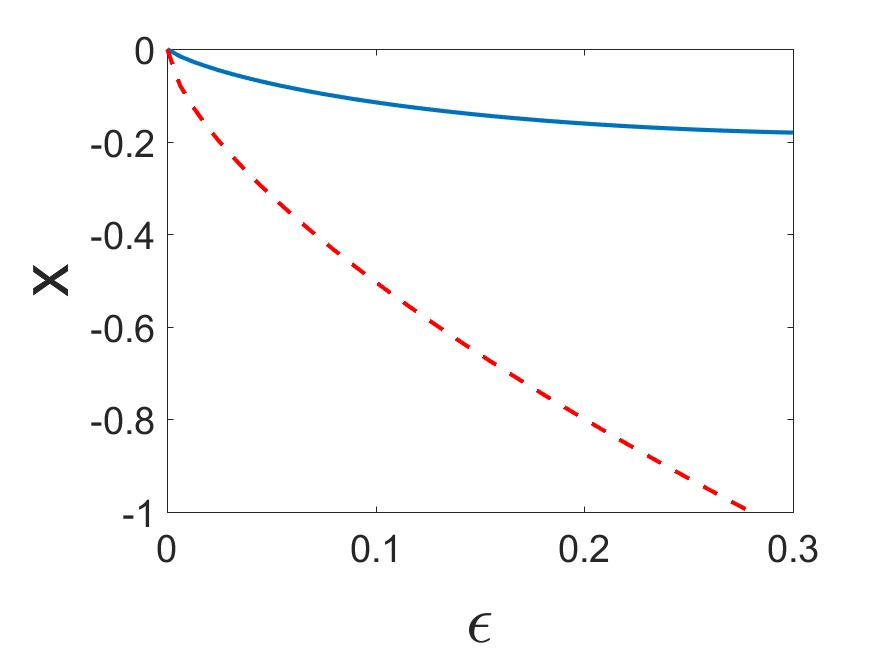
\includegraphics[width=.7\linewidth]{conclusion/slowcomp.jpg}
\caption{Comparison between the slow tipping points across $\epsilon$. The blue solid line is the non-smooth tipping points where the red dotted line is the smooth tipping points.}
\label{fig:slow_comp}
\end{figure}

\indent For oscillatory forcing with $A\not = 0$ and static parameter values with $\epsilon=0$, we compare the non-smooth bifurcation, $\mu_{\text{osc}} = \frac{4|A|}{\pi \Omega}$, to the smooth bifurcation, $\mu_{\text{sm+osc}}=\frac{A^2}{2\Omega^2}$. Here we have a sense of the strength of each case directly from the functions in terms of $\Omega^{-1}$, the non-smooth has a linear response whereas the smooth has a quadratic response. This appears clearly in figure~\ref{fig:osc_comp} where we see that the advanced bifurcation in the non-smooth case is significantly greater than that of the smooth case. This means that the non-smooth bifurcation causes the oscillations to advance the bifurcation much further away as opposed to the smooth bifurcation. Here this also indicates that the effects of the non-smooth effects are stronger than that of the smooth effects.

\begin{figure}[H]
\centering
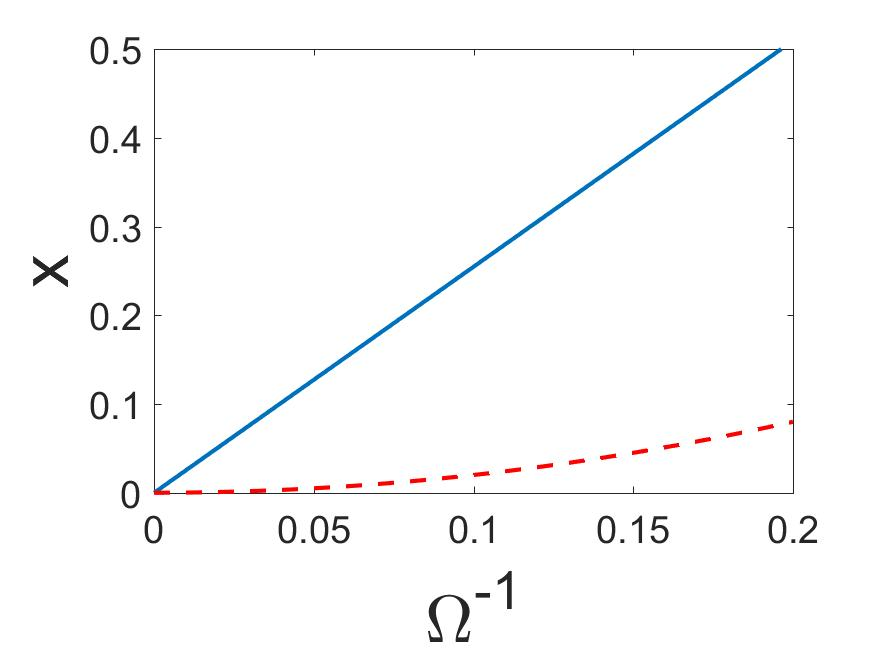
\includegraphics[width=.7\linewidth]{conclusion/osccomp.jpg}
\caption{Comparison between the oscillatory bifurcation across $\Omega^{-1}$ for $A=2$. The blue solid line is the non-smooth case where the red dotted line is the smooth case.}
\label{fig:osc_comp}
\end{figure}

\indent When we combine these mechanisms, we compare the non-smooth tipping point , $\mu_{\text{mixed}}=w(\Omega,A) \mu_{\text{smooth}}+\mu_{\text{osc}}$ with weight $w(\Omega,A)=(\frac{2|A|}{\pi\Omega})^{1/3}$, to the smooth tipping point, $\mu_{\text{smooth}}+\mu_{\text{sm+osc}}$. The case where the mixed approximation take the form of $\mu_{\text{slow}}$ for $\Omega\to\infty$ has already been discussed above so we do not consider this here. It is important to note that although we see a similar form between these two, the weight in the non-smooth tipping point is dependent on both $A$ and $\Omega$ so it has significant influence on the value for different frequencies. This is shown in figure~\ref{fig:mixed_comp} for $\epsilon$ varying in (a) and $\Omega$ varying in (b). In (a), since the weight $w(\Omega,A)<1$ for $A<O(\Omega)$, then the slope of non-smooth influence is smaller than the slope of smooth influence. We also notice the intercept for the non-smooth influence being significantly larger corresponding to the oscillatory bifurcation $\mu_{\text{osc}}$ being larger than $\mu_{\text{sm+osc}}$. Together, these indicate that the non-smooth bifurcation has a stronger advanced tipping while the curves are both positive, and a smaller delayed tipping when both curves are negative. In (b), the effect of the changing weight $w(\Omega,A)$ is most clear and we see the advanced tipping being quite strong for mid-range $\Omega$. It is also clear the non-smoothness of the model causes the approximation $\mu_{\text{mixed}}$ to fail for $\Omega\to\infty$. This case is analogous to when $\lambda>1$ from the one component analysis and allows us to refer back to the slowly varying problem with $\epsilon>0$ and $A=0$ for $\Omega\to\infty$. For both plots, we conclude the non-smooth effects are stronger than the smooth effects even under the mixed case.

\begin{figure}[H]
\centering
\begin{subfigure}{.5\textwidth}
 \centering
 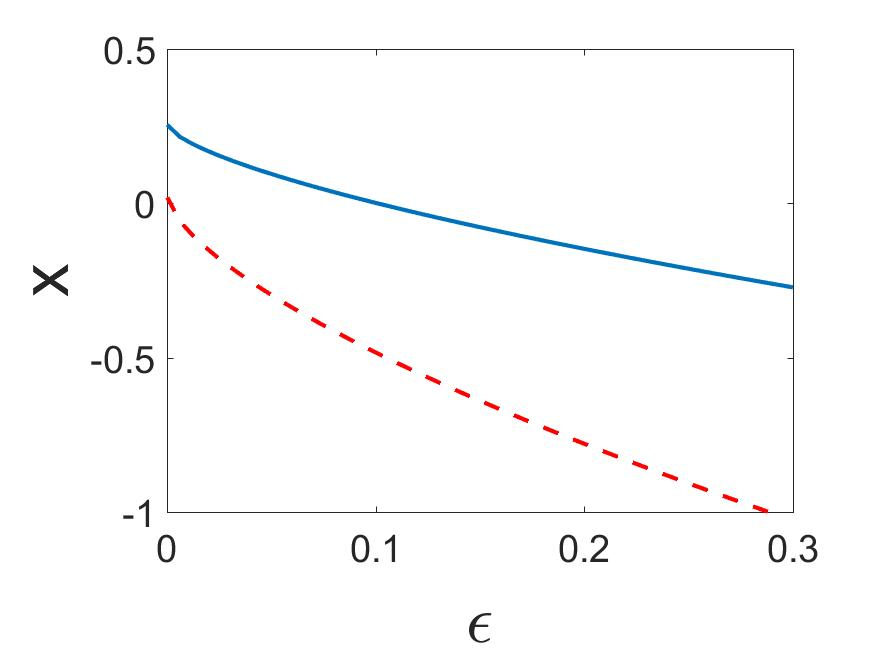
\includegraphics[width=\linewidth]{conclusion/mixedcomp_eps.jpg}
 \caption{}
\end{subfigure}%
\begin{subfigure}{.5\textwidth}
 \centering
 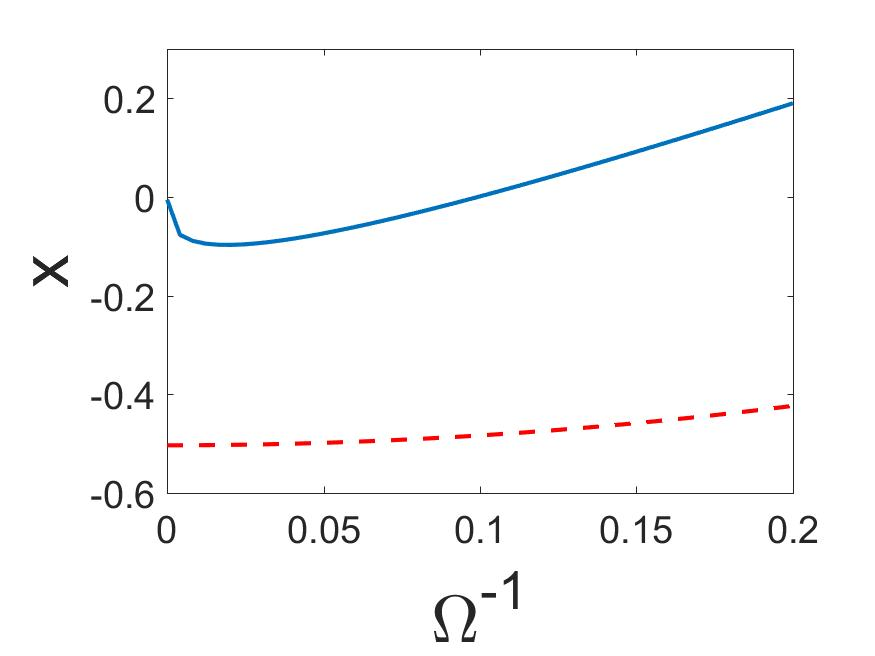
\includegraphics[width=\linewidth]{conclusion/mixedcomp_omega.jpg}
 \caption{}
\end{subfigure}
\caption{Comparison between the mixed tipping in (a) with a fixed $\Omega^{-1}=.1$ and (b) with a fixed $\epsilon=.1$. The blue solid line is the non-smooth case where the red dotted line is the smooth case.}
\label{fig:mixed_comp}
\end{figure}

\indent  These results give insight into the hysteresis behavior of the Stommel model and the less studied realm of non-smooth dynamics. The main approach used asymptotic expansions as well as the methods of multiple scales to identify reduced equations and to find asymptotic solutions to the models. We found that with oscillatory forcing, the reduced equations have an expression dependent on the relative size of the solution to the amplitude of oscillation. In the smooth version of this problem, this type of behavior was not present and considering a case-by-case argument was not necessary. We also discovered that linking the slow variation $\epsilon$ and the frequency $\Omega$ gives important insight into how the system behaves. The methods developed for finding tipping points in the one component model \eqref{eq:oneD_canonical} gave good approximations with the numerical results. Due to the many similarities to the two component system \eqref{eq:twoD_canonical} we were able to modify the same analysis to find the tipping points here as well. We also anticipate the non-smooth bifurcation of the Stommel model to have a stronger influence on the solution than the smooth bifurcation.

\indent Future work would need to be done on cases where $\Omega\sim O(1)$ or smaller. This case is qualitatively different as slow oscillations may have dramatic contributions to the dynamics. These effects are also seen from the analysis where low frequency oscillations no longer allow for asymptotic expansions in terms of $\Omega^{-1}$ and no longer fall under our assumptions to integrate with $T_1$ and $T_2$. Hence this case can influence tipping in a way we hadn't explored in this paper, we show an example of this in figure~\ref{fig:low_freq}. Also, large amplitude behavior $A>O(1)$ can force an additional rescaling before any familiar approaches hold which is seen in figure~\ref{fig:large_amp}. These cases were mentioned but have yet to be performed on this model, although both have been studied around the smooth case in \cite{zhu2015tipping}. It is possible that they could have some surprising results in the non-smooth case. Together, these could help to further classify the tipping behavior for the variety of cases in real world ocean dynamics.

\begin{figure}[H]
\centering
\begin{subfigure}{.5\textwidth}
 \centering
 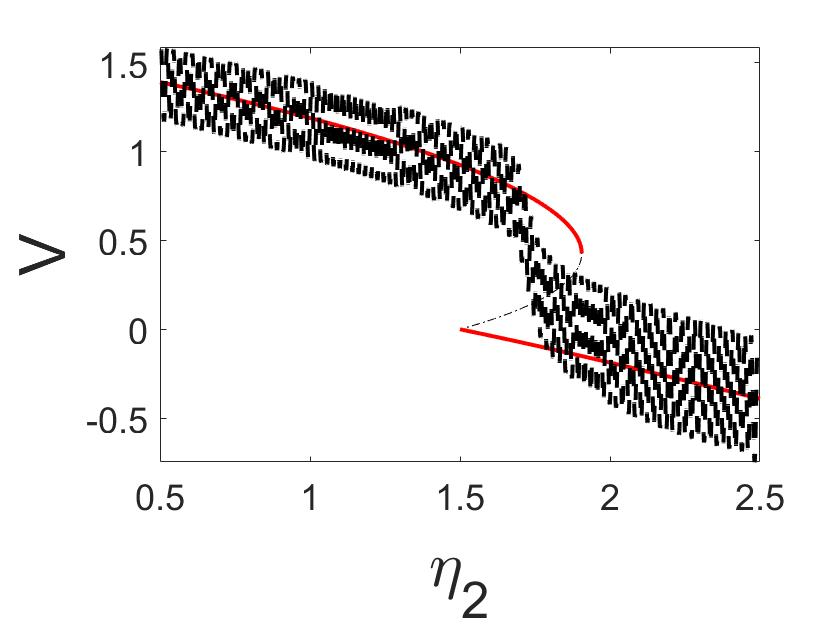
\includegraphics[width=\linewidth]{conclusion/low_freq_V.jpg}
 \caption{}
\end{subfigure}%
\begin{subfigure}{.5\textwidth}
 \centering
 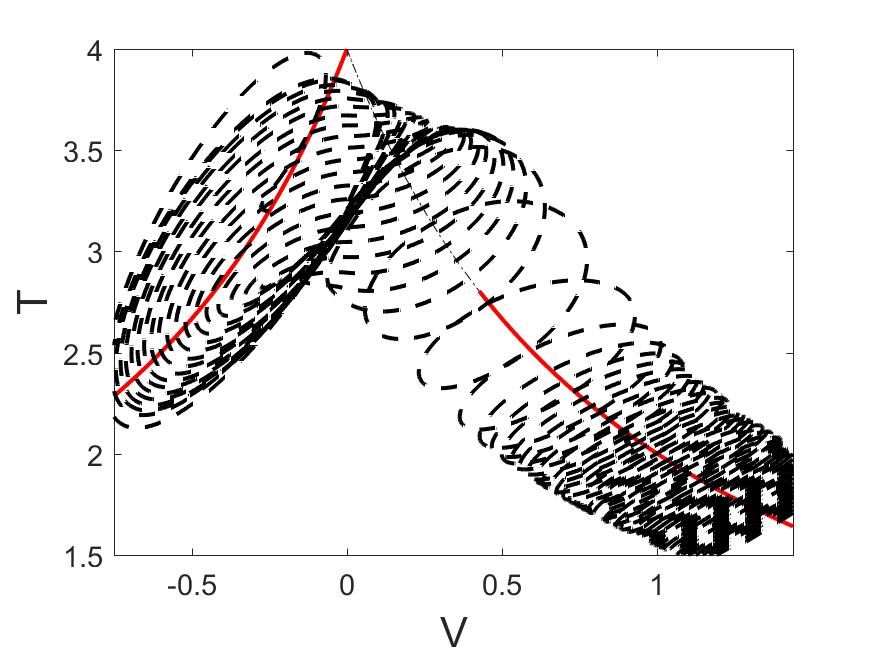
\includegraphics[width=\linewidth]{conclusion/low_freq_T.jpg}
 \caption{}
\end{subfigure}
\caption{Low Frequency: Model parameters are $\epsilon=.01$, $A=B=1$ and $\Omega=3$.}
\label{fig:low_freq}
\end{figure}

\begin{figure}[H]
\centering
\begin{subfigure}{.5\textwidth}
 \centering
 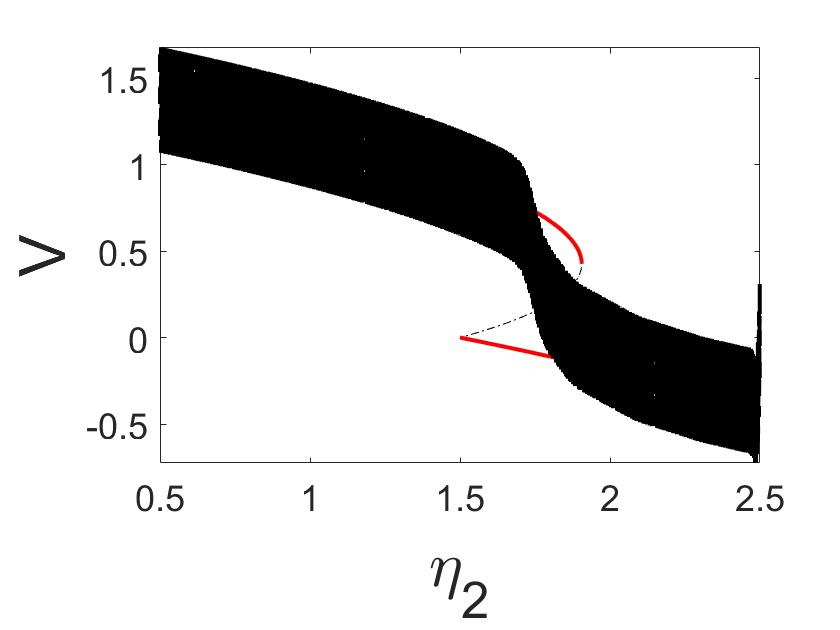
\includegraphics[width=\linewidth]{conclusion/large_amp_V.jpg}
 \caption{}
\end{subfigure}%
\begin{subfigure}{.5\textwidth}
 \centering
 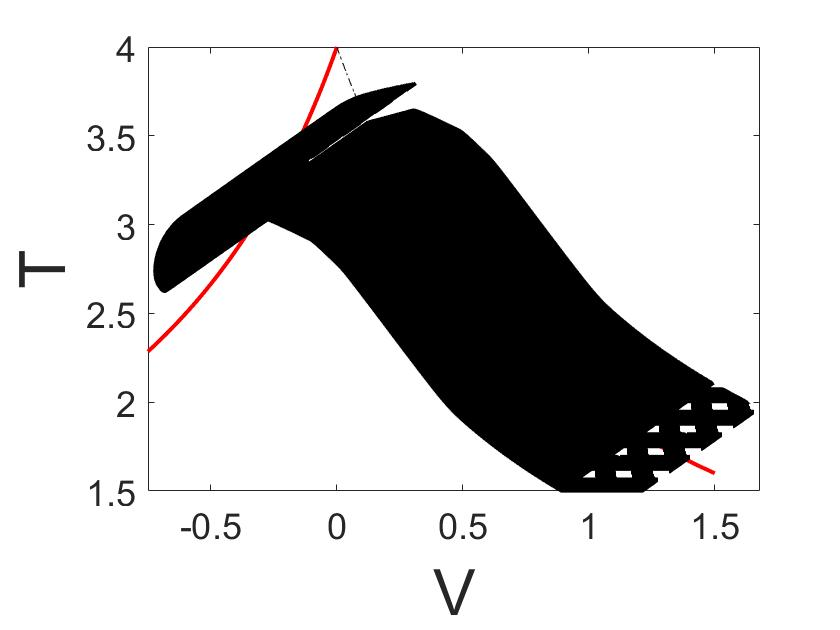
\includegraphics[width=\linewidth]{conclusion/large_amp_T.jpg}
 \caption{}
\end{subfigure}
\caption{Large Amplitude: Model parameters are $\epsilon=.01$, $A=B=300$ and $\Omega=1000$.}
\label{fig:large_amp}
\end{figure}

\indent Lastly, we considered only deterministic behavior throughout this analysis but there are many reasons to incorporate stochastic elements into the Stommel model as well, see \cite{lorenzo2012role}. From \cite{zhu2015tipping} it is concluded that stochastic forcing has elements of both early bifurcations and delayed tipping and thus a natural follow-up to the analysis in this thesis. We could consider stochastic forcing with

\begin{equation}\label{eq:stochastic}
\begin{aligned}
\dot{V} & = \eta_1-\eta_2+\eta_3(T-V)-T-V|V|+A\xi_1(t), \\
  \dot{T}   & = \eta_1-T(1+|V|)+B\xi_2(t), \\
 \dot{\eta_2} & = -\epsilon\\
 V(0)=&V^0,\quad T(0)=T^0, \quad \eta_2(0)={\eta_2}^0,
\end{aligned}
\end{equation}

where $\xi_i(t)$ is standard Gaussian noise with mean 0 and variance $t$ and initial conditions centered on the lower branch. This is shown in figure~\ref{fig:stochastic} and it is clear that a completely separate analysis is needed.

\begin{figure}[H]
\centering
\begin{subfigure}{.5\textwidth}
 \centering
 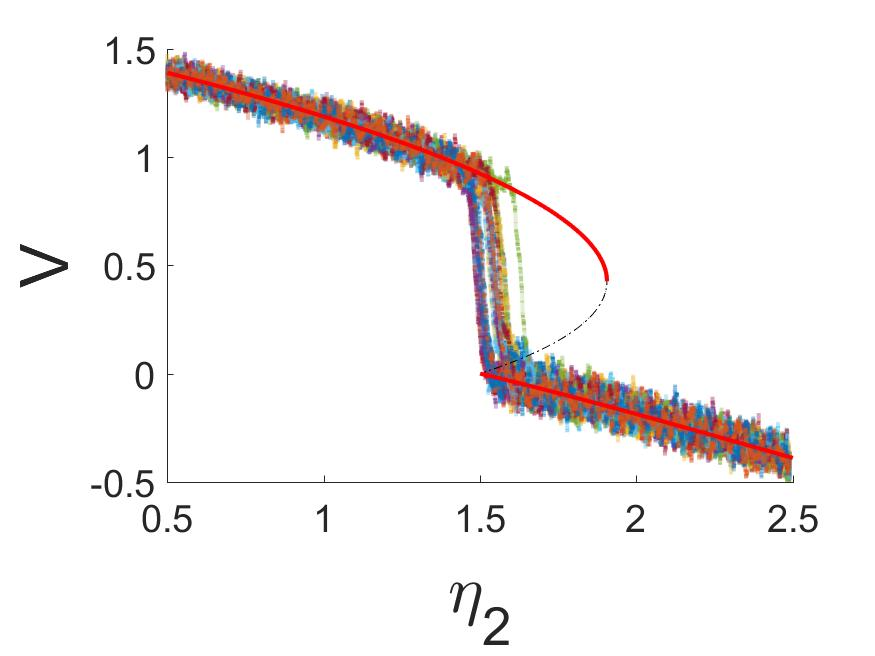
\includegraphics[width=\linewidth]{conclusion/stochastic_V.jpg}
 \caption{}
\end{subfigure}%
\begin{subfigure}{.5\textwidth}
 \centering
 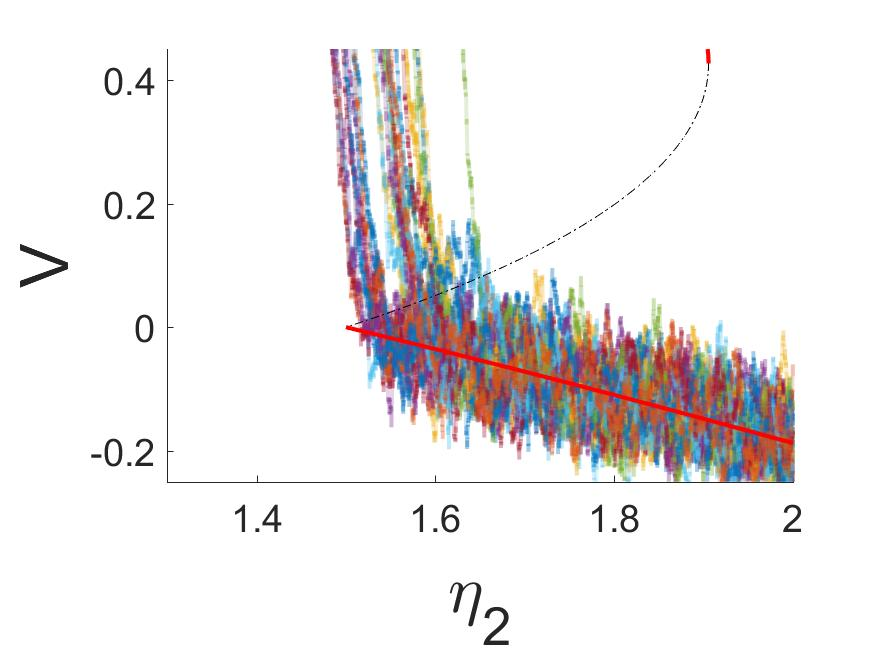
\includegraphics[width=\linewidth]{conclusion/stochastic_V_zoom.jpg}
 \caption{}
\end{subfigure}
\begin{subfigure}{.5\textwidth}
 \centering
 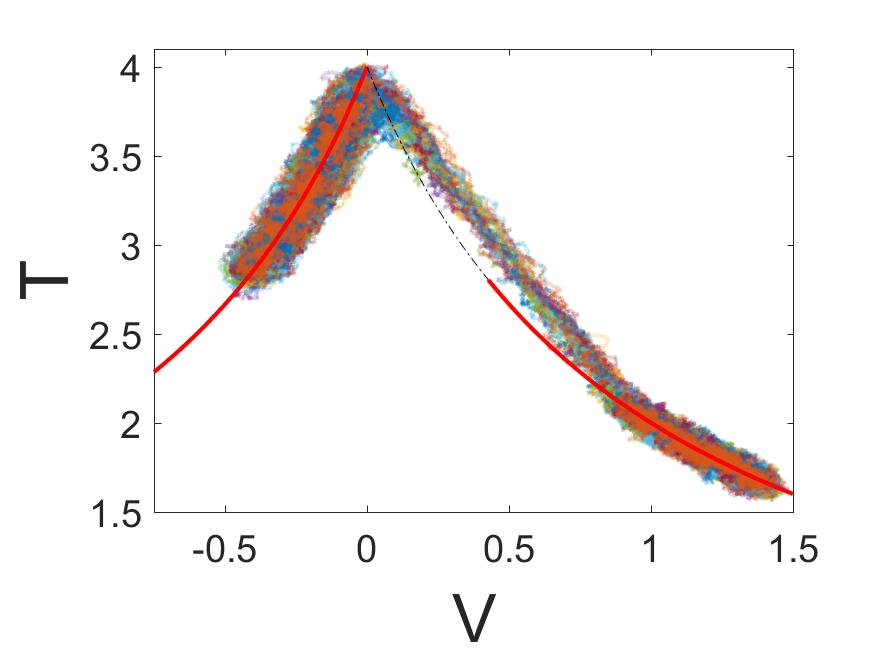
\includegraphics[width=\linewidth]{conclusion/stochastic_T.jpg}
 \caption{}
\end{subfigure}%
\begin{subfigure}{.5\textwidth}
 \centering
 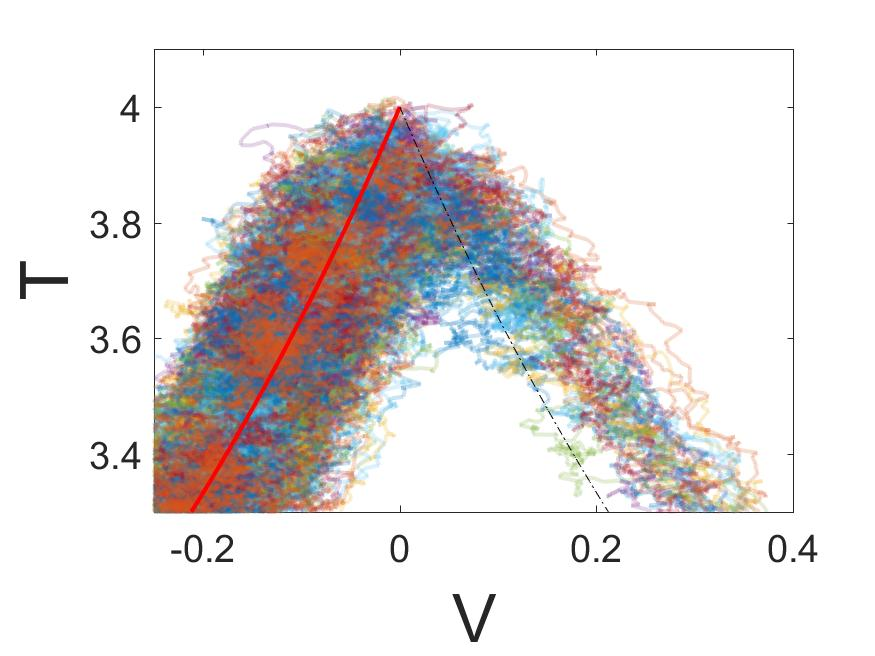
\includegraphics[width=\linewidth]{conclusion/stochastic_T_zoom.jpg}
 \caption{}
\end{subfigure}
\caption{Stochastic: In (a) many realizations of the numerical solution for $V$ in \eqref{eq:stochastic} are given with model parameters $\eta_1=4$, $\eta_3=.375$, $\epsilon=.01$ and $A=B=.7$. In (b) a zoom in closer to the non-smooth bifurcation region can be seen. In (c) we have the realizations over the standard equilibrium plot for $V$ vs. $T$. In (d) a zoom of the bifurcation area is shown.}
\label{fig:stochastic}
\end{figure}